\chapter{Solução Proposta}\label{cap:solucao}

Uma vez que o conhecimento teórico necessário para o entendimento completo do trabalho já foi apresentado, neste capítulo será definida a solução proposta.

A solução desenvolvida consiste em um algoritmo que analisa imagens de vídeo de um estacionamento descoberto e determina o número de vagas livres na imagem, além da sua localização aproximada. O sistema funciona bem em imagens de menor qualidade, mas é necessário que as imagens que compõem o vídeo estejam no espaço de cor RGB. Chamaremos a solução apresentada a seguir de \textit{Dectector de vagas em estacionamento} ou \textit{DVE}. A partir deste momento no trabalho, referências ao programa se referem ao \textit{DVE}.

O trabalho se preocupa em cumprir os critérios definidos no Capítulo \ref{cap:trabalhos}. Além disso, o sistema foi desenvolvido de forma que pudesse processar as imagens adquiridas de forma mais próxima possível do tempo real, causando o mínimo de atrasos para o processamento de quadros subsequentes do vídeo.

O sistema recebe como entrada um vídeo em cores capturado em um certo ângulo e um vetor de regiões de interesse no vídeo. A saída do \textit{DVE} a cada quadro é o número de vagas livres em cada região de interesse no vídeo.

A Figura \ref{fig:fluxograma} contém um fluxograma que mostra as etapas do processamento de cada quadro do vídeo adquirido. No decorrer deste capítulo cada um desses passo será discutido com mais detalhes.

\begin{figure}
	\centering
	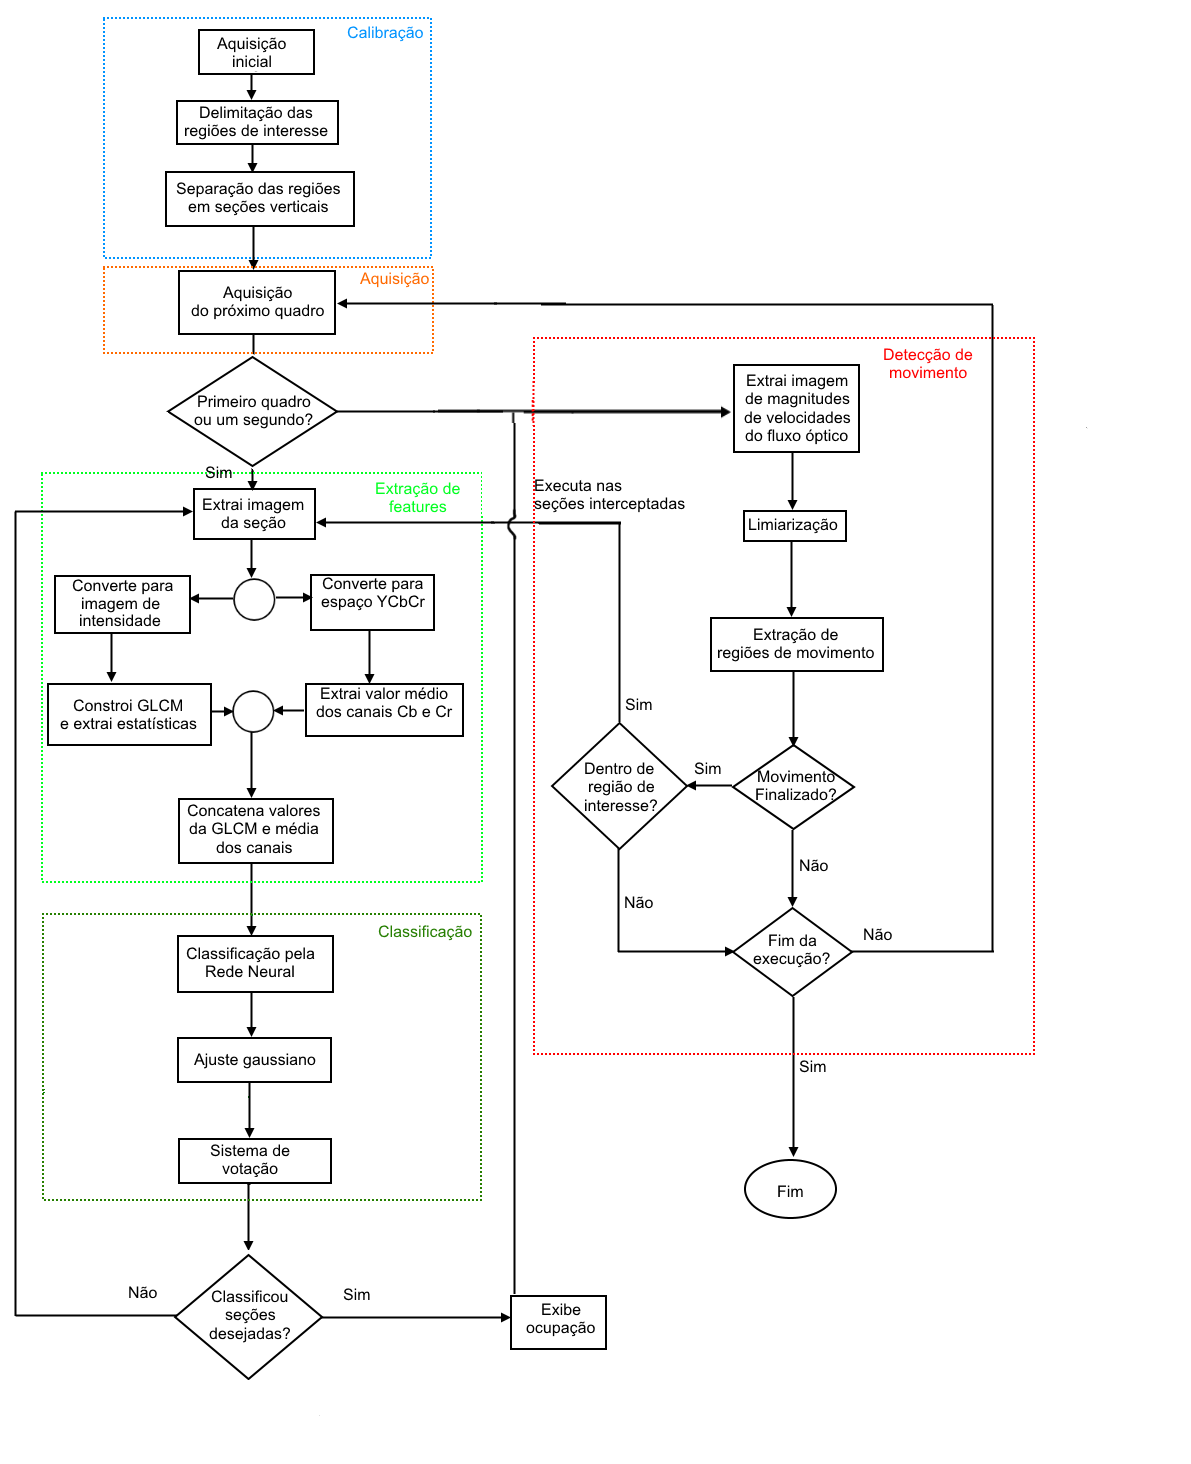
\includegraphics[width=1.2\textwidth]{fluxograma}
	\caption{Um fluxograma com o funcionamento geral do \textit{DVE}}
	\label{fig:fluxograma}
	\centering
\end{figure}



\section{Aquisição}\label{sec:aquisicao}

Uma câmera montada em um poste de luz ou outro ponto similar captura as imagens utilizadas pelo \textit{DVE}. A câmera é montada de forma que o seu campo de visão contenha o máximo de vagas possível, porém que ainda seja possível visualizar o asfalto das vagas desocupadas e ocorra o mínimo de oclusão de veículos. A Figura \ref{fig:aquisicao} mostra um quadro de uma aquisição em ângulo ideal.

\begin{figure}[!ht]
	\centering
	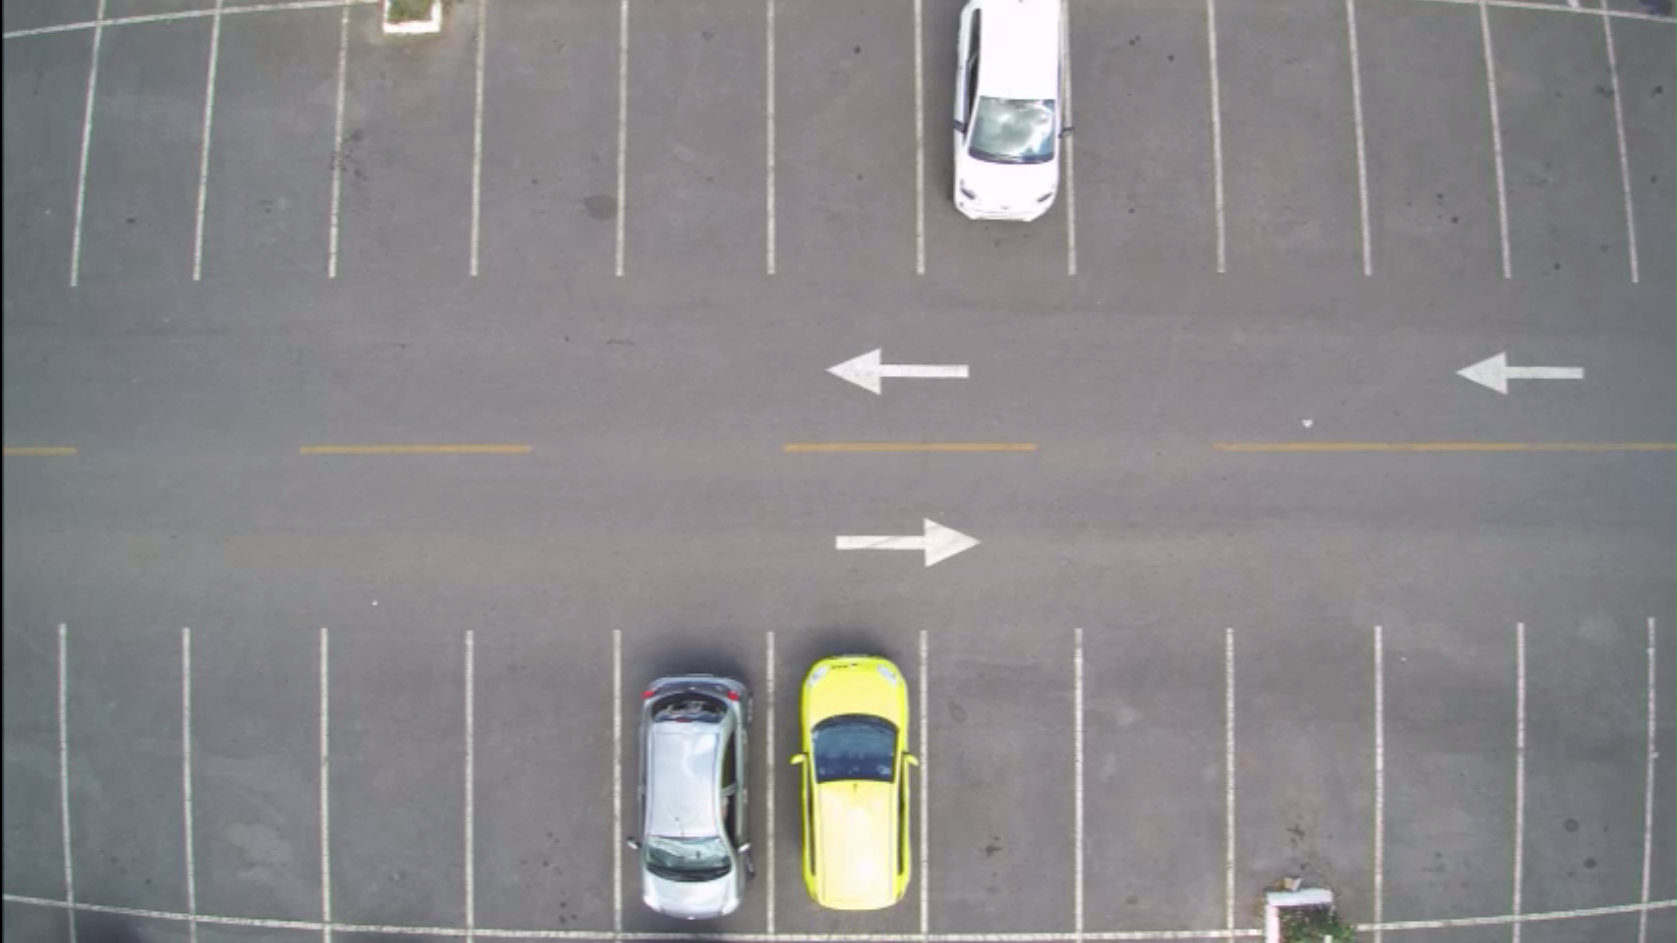
\includegraphics[width=8cm]{Vazio3}
	\caption{Um quadro de um vídeo adquirido por uma câmera do sistema}
	\label{fig:aquisicao}
	\centering
\end{figure}

Neste trabalho, a preocupação foi implementar um programa que analisa as imagens de uma única câmera de vídeo. Em uma aplicação no mundo real, diversas câmeras seriam instaladas para aumentar a cobertura do estacionamento. Neste caso, cada vídeo seria processado por uma cópia diferente do sistema, responsável pela área coberta pela câmera correspondente. As saídas de cada cópia do programa correspondem a ocupação das vagas em um setor diferente do estacionamento.

\section{Regiões de Interesse}\label{sec:ROIs}

No momento da instalação do \textit{DVE}, é necessário definir um número qualquer de regiões de interesse(\textit{Regions of interest} ou ROIs). Essas regiões determinam a área da imagem onde existem vagas. Além de determinar as regiões, deve-se informar ao programa o número de vagas existente em cada região de interesse.

As ROIs devem ser retangulares e determinadas de forma a não haver interseção entre as regiões, como exemplificado na Figura \ref{fig:ROIs} que mostra as regiões determinadas para o quadro da Figura \ref{fig:aquisicao}.

\begin{figure}
	\centering
	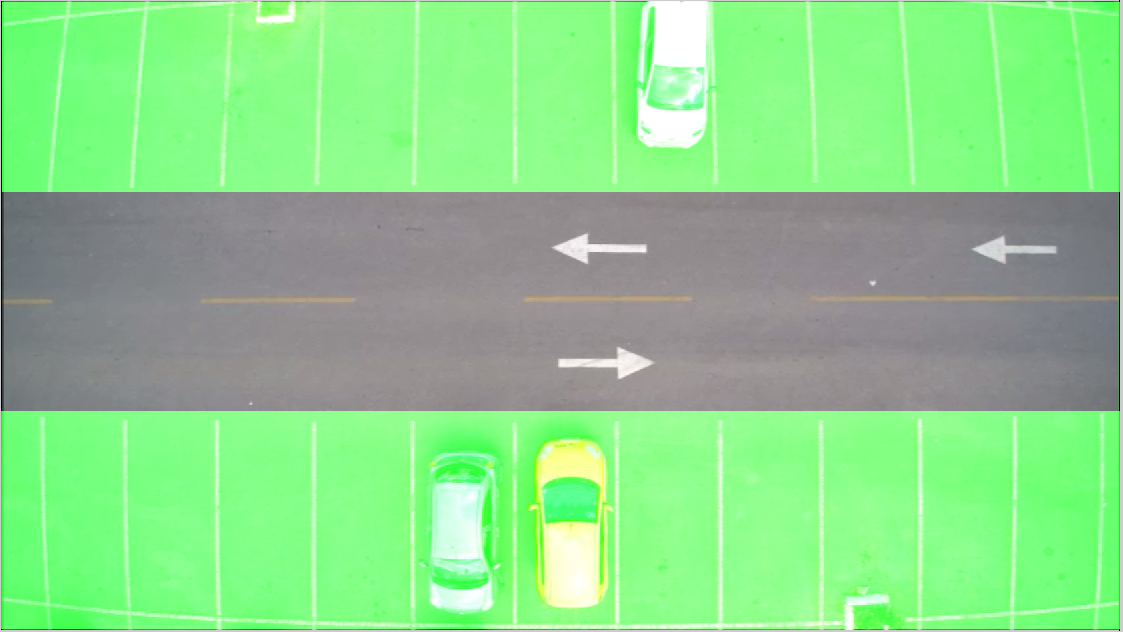
\includegraphics[width=8cm]{ROIs}
	\caption{O mesmo quadro da Figura \ref{fig:aquisicao}, depois de definidas as regiões de interesse, marcadas de verde.}
	\label{fig:ROIs}
	\centering
\end{figure}

Depois de determinadas as regiões de interesse, cada uma das regiões é dividida em um número igual de seções verticais como ilustrado na Figura \ref{fig:secoesVerticais}. Como as vagas não são determinadas individualmente no momento da instalação do \textit{DVE}, é necessário que seja feita alguma divisão das ROIs. Cada uma destas seções verticais é classificada separadamente em uma etapa futura do processamento. O resultado da classificação de cada seção de uma ROI determina um vetor $v$ de $n$ elementos, onde $n$ é o número de seções em que a região foi dividida e cada elemento indica a ocupação de uma seção, sendo o valor $1$ correspondente a uma seção ocupada e o valor $2$ correspondente a uma seção livre. Através da análise deste vetor é que o \textit{DVE} determina o número de vagas livres em cada região. Munido do número de vagas que cada região contém e um valor aproximado do número de seções que um carro ocupa, o programa estima quantas vagas estão ocupadas, e encontra o número de vagas livres através de simples subtração e a posição aproximada destas vagas através da posição das seções livres no vetor.

\begin{figure}
	\centering
	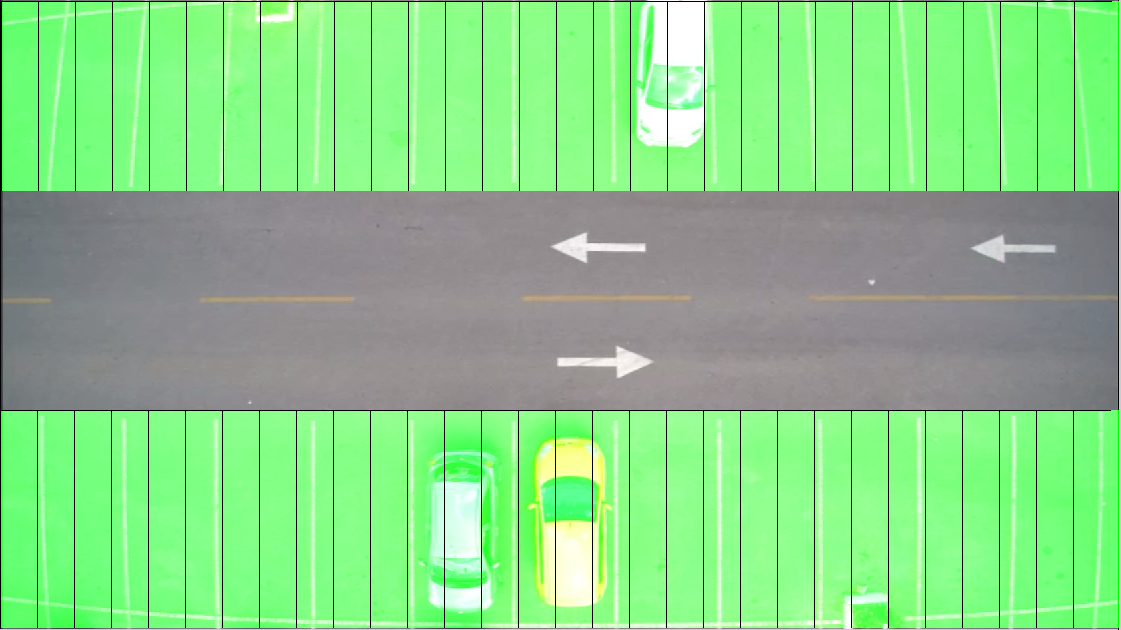
\includegraphics[width=8cm]{Secoes}
	\caption{As ROIs determinadas na Figura \ref{fig:ROIs} separadas em trinta seções verticais que ainda não foram classificadas. Nesta etapa os vetores $v$ de cada região é composto de trinta valores $2$.}
	\label{fig:secoesVerticais}
	\centering
\end{figure}


Uma vez que as regiões de interesse foram definidas e divididas em seções, a etapa de configuração inicial é finalizada e o programa pode iniciar o processo de determinação da ocupação das vagas. 

\section{Classificação das seções} \label{sec:classificacao}

O primeiro passo na execução do \textit{DVE} depois da configuração inicial é a classificação de cada uma das sessões verticais criadas na imagem. Essa classificação é feita assim que a execução começa, no primeiro quadro do vídeo e é repetida a cada segundo de execução do programa. Além disso, quando se detecta movimento em uma das ROIs as sessões interceptadas pelo movimento detectada são classificadas. O processo de detecção de movimento e determinação das sessões a serem classificadas excepcionalmente é detalhado na Seção \ref{sec:sub:regioesmovimento}.

Para que seja feita a extração das caracterísiticas e a classificação de uma seção, uma imagem $I_s$ é extraída do quadro de vídeo original capturado.Essa imagem corresponde à fração do quadro contida dentro dos limites da seção a ser analisada. A extração de $I_s$ consiste simplesmente em copiar os valores da matriz que representa o quadro que estavam dentro das bordas da seção em uma nova matriz de dimensões iguais às da seção. A Figura \ref{fig:imgSecao} mostra um exemplo de uma $I_s$. Cada uma dessas imagens é submetida separadamente ao processo de classificação.

\begin{figure}
	\centering
	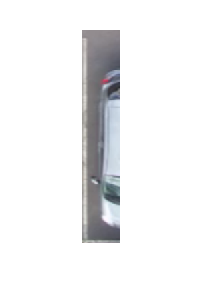
\includegraphics[height=5cm]{imgSecao}
	\caption{Uma imagem correspondente a uma das seções verticais definidas.}
	\label{fig:imgSecao}
	\centering
\end{figure}


\subsection{Extração de características}\label{sec:extracao}

O processo de classificação de uma seção começa com a extração das características que definem o padrão de cada classe e a criação do vetor de entrada da rede neural artifical. Dois conjuntos de características principais são extraídos: as quatro medidas extraídas da GLCM da imagem apresentadas na Seção \ref{sec:GLCM} e dois valores que descrevem a crominância azul e vermelha da seção.

Para a extração da GLCM é preciso primeiro obter uma imagem de níveis de cinza que represente $I_s$. Para isso, a imagem é convertida para o espaço $YCbCr$ como descrito na Seção \ref{sect:sub:ycbcr}. A imagem referente ao canal $Y$ resultante é uma imagem de intensidade e por isso é utilizada para o cálculo da GLCM. Como mencionado na Seção \ref{sec:GLCM}, a construção é feita com base na vizinhança a direita de cada \textit{pixel} da imagem. Cada valor dentre os 256 possíveis é dividido dentro de 8 níveis distintos, e sempre que um valor presente em nível $N$ aparece a direita de um valor de um nível $M$, o elemento $(N,M)$ da GLCM é incrementado. A Figura \ref{fig:GLCM} mostra esse processo.

Uma vez construída a GLCM referente a sessão, quatro medidas estatísticas são extraídas: contraste, correlação, energia e homogeneidade. Essas medidas são calculadas pelas Equações \ref{eq:Contraste}, \ref{eq:Correlacao}, \ref{eq:Energia} e \ref{eq:Homo} respectivamente. Esses valores formam um vetor $g = (\text{\textit{contraste, correlação, energia, homogeneidade}})^T$ que é parte da entrada final da rede neural artificial. O vetor na Equação \ref{eq:exemploGLCM} representa o vetor $g$ da Figura \ref{fig:imgSecao}.

\begin{equation}
\centering
	g = \begin{pmatrix}
	0,2170\\0,9208\\0,2084\\0,9019
	\end{pmatrix}
\centering
\label{eq:exemploGLCM}
\end{equation}

As outras duas características extraídas de cada sessão vêm dos canais $Cb$ e $Cr$ de $I_s$. A média de valores da matriz de cada canal é calculada através da Equação \ref{eq:media}. Onde $N$ é o número total de \textit{pixels} de $I_s$ e $v_i$ é o valor do \textit{i-ésimo pixel}. Esses valores então formam o vetor $c = (M_{Cb}, M_{Cr})^T$.

\begin{equation}
	M = \frac{\sum_{i=1}^N v_i}{N}
\label{eq:media}
\end{equation}

O vetor $c$ da Figura \ref{fig:imgSecao} é:

\begin{equation}
\centering
\centering
	c = \begin{pmatrix}
	130,7157\\127,0190
	\end{pmatrix}
\centering
\centering
\label{eq:exemploCrominancia}
\end{equation}


Essas características foram escolhidos por terem se mostrado suficientemente descritivas e distintivas após uma análise de um conjunto de 90 imagens. As Figuras \ref{fig:histContraste}, \ref{fig:histCorrelacao},  \ref{fig:histEnergia}, \ref{fig:histHomo},  \ref{fig:histCb} e \ref{fig:histCr} mostram histogramas que descrevem a distribuição das características no conjunto de imagens. Em cada um dos gráficos, o eixo $x$ correspondente a valores obtidos para caracterísitica em questão e o eixo $y$ indica o número de imagens que exibiram aquele valor. As barras azuis são referentes as imagens de carros ou vagas ocupadas e as barras vermelhas referentes a vagas vazias.

\begin{figure}
	\centering
	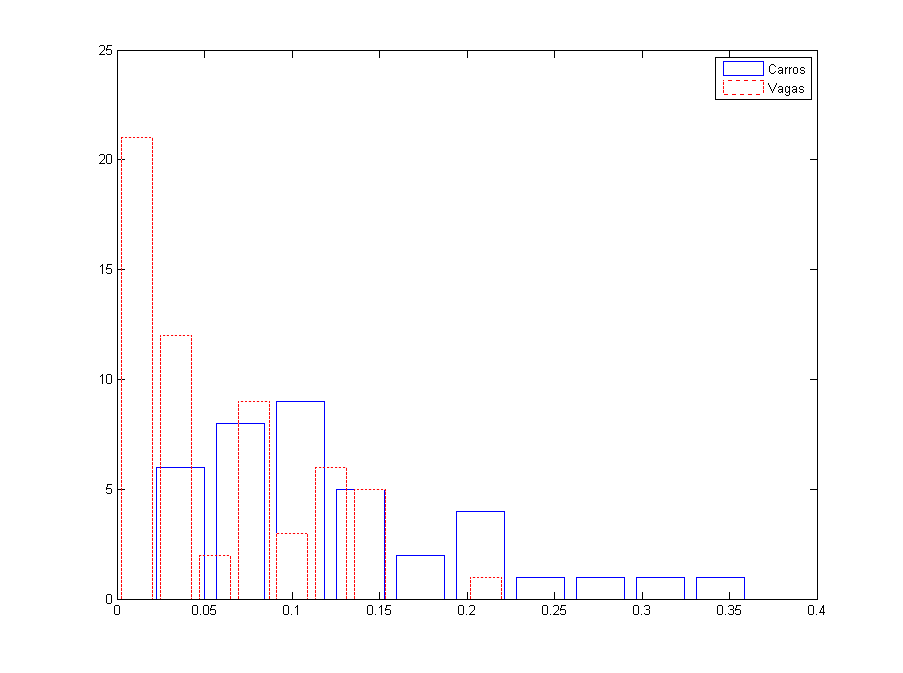
\includegraphics[width=11cm]{Contraste}
	\caption{O histograma referente aos valores de contraste no conjunto analisado. Apesar de haver bastante sobreposição dos valores ainda é possível ver que há pouco ou nenhuma ocorrência de vagas após um certo valor.}
		\label{fig:histContraste}
	\centering
\end{figure}

\begin{figure}
	\centering
	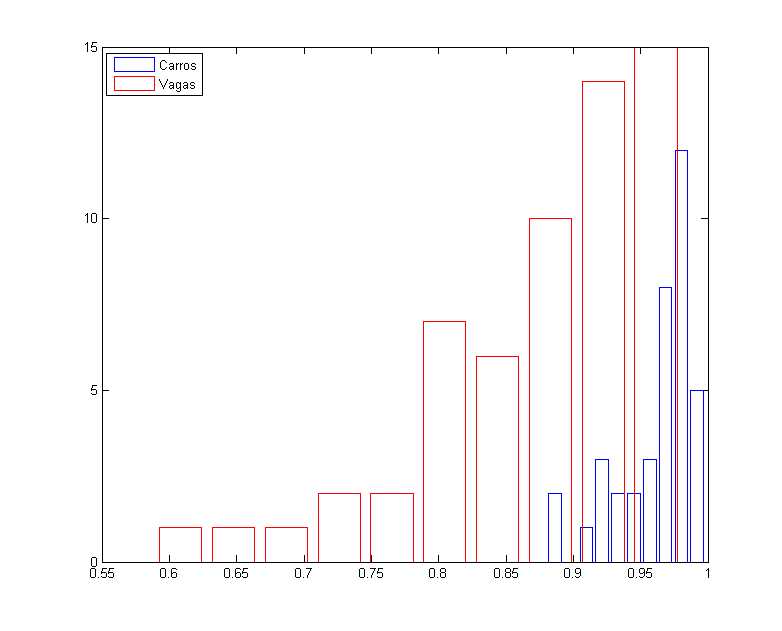
\includegraphics[width=11cm]{Correlacoes}
	\caption{O histograma referente aos valores de correlação no conjunto analisado. Aqui é possível ver um limiar inferior para a classe dos carros. Valores abaixo deste limiar provavelmente são vagas livres.}
		\label{fig:histCorrelacao}
	\centering
\end{figure}

\begin{figure}
	\centering
	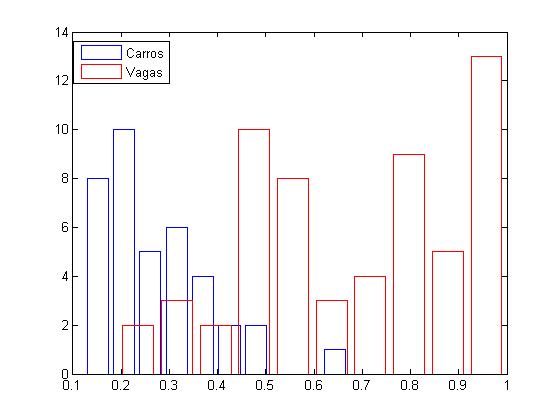
\includegraphics[width=11cm]{Energia}
	\caption{O histograma referente aos valores de energia no conjunto analisado. Há um ponto de divisão entre as duas classes, com pouca sobreposição de valores entre as classes.}
		\label{fig:histEnergia}
	\centering
\end{figure}

\begin{figure}
	\centering
	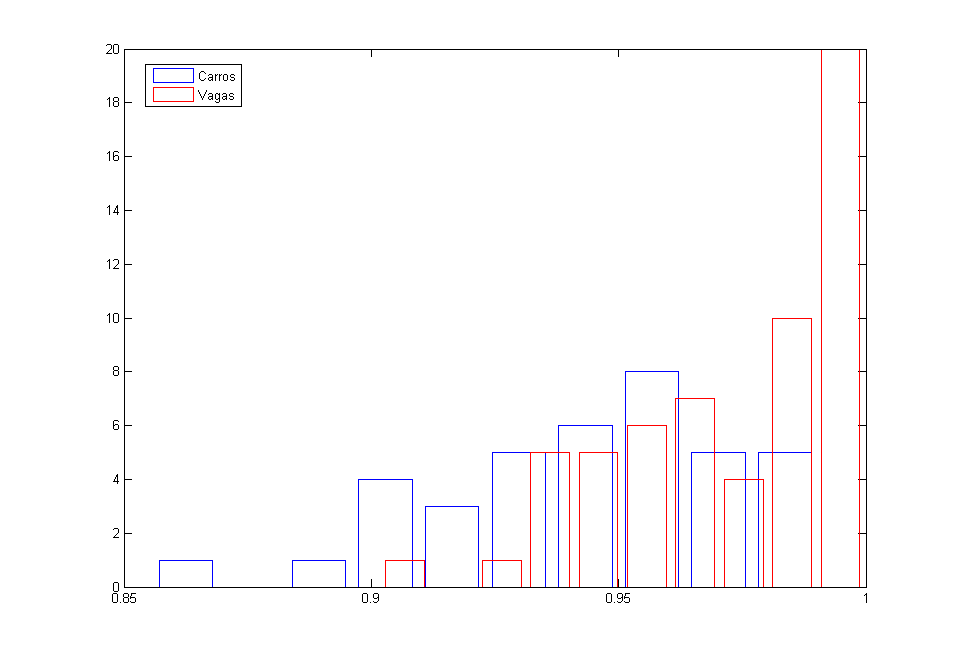
\includegraphics[width=11cm]{Homogeneidade}
	\caption{O histograma referente aos valores de homogeneidade no conjunto analisado. Esse gráfico mostra mais sobreposição do que os anteriores, mas ainda contém bastante informação sobre a classe das vagas. }
	\label{fig:histHomo}
	\centering
\end{figure}

\begin{figure}
	\centering
	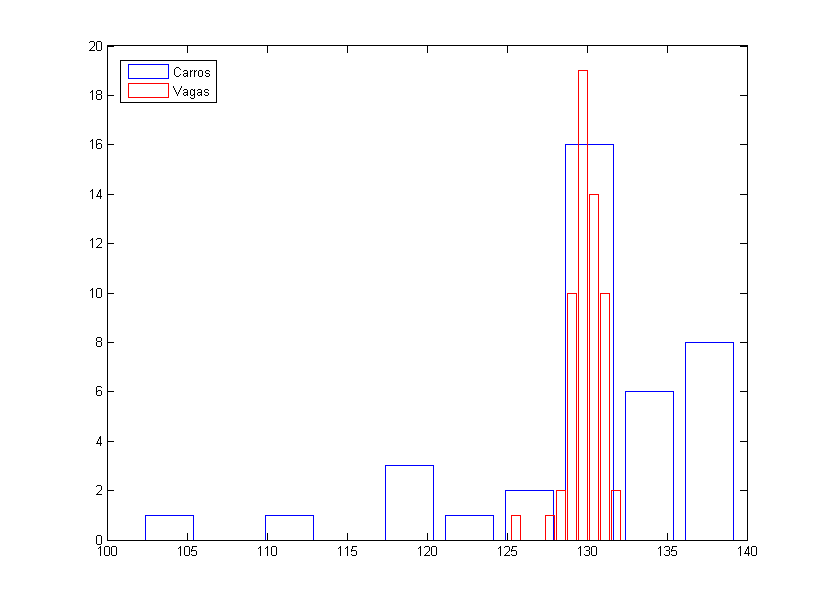
\includegraphics[width=11cm]{CrominanciaAzul}
	\caption{O histograma referente aos valores médios de crominância azul no conjunto analisado. Apesar de haver alta variedade nos valores encontrados nas imagens de carros, as imagens de faixa possuem valores médios em uma faixa estreita. }
		\label{fig:histCb}
	\centering
\end{figure}

\begin{figure}
	\centering
	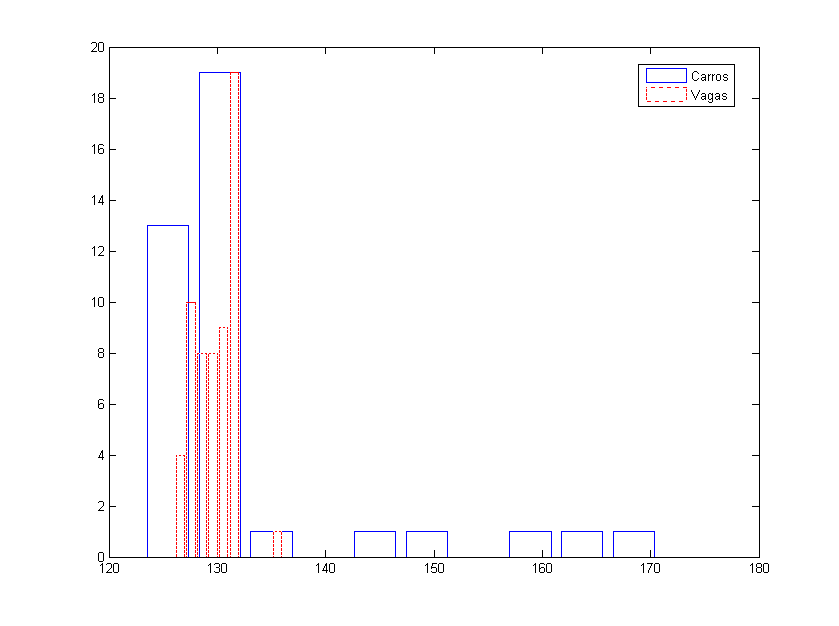
\includegraphics[width=11cm]{CrominanciaVermelha}
	\caption{O histograma referente aos valores médios de crominância vermelha no conjunto analisado, mostrando comportamento semelhante ao histograma de valores médios de crominância azul. }
		\label{fig:histCr}
	\centering
\end{figure}


\subsection{Classificação da rede neural artificial}

Depois de extraídas as características das imagens e construídos os vetores $g$ e $c$ com os valores das características, a entrada para a rede neural artificial é construída. O vetor de entrada $x_s$ referente a seção a ser classificada é a concatenação de $g$ e $c$ de forma que:

\begin{equation}
	x_s = (\text{\textit{contraste, correlação, energia, homogeneidade}}, M_{Cb}, M_{Cr})^T
\end{equation}

O vetor $x_s$ é alimentado à rede neural artificial que retorna um vetor $y_s$ de saída que possue dois elementos com valores reais entre $0$ e $1$. Esses valores sempre somam $1$ e representam o grau de certeza que a rede tem de que a o $x_s$ representa um elemento da classe correspondente ao seu índice. Isto é, o primeiro elemento, $y_s(1)$ representa o grau de certeza que a rede tem que a entrada pertence à classe $1$, os carros, e o segundo elemento, $y_s(2)$ representa o grau de certeza que a rede tem que a entrada pertence à classe $2$, das vagas livres. O vetor $y_s$ é armazenado e processado futuramente para decidir a classe final a que a vaga pertence. Os vetores da Equação \ref{eq:vetoresRede} correspondem ao s vetores $x_s$ e $y_s$ da seção mostrada na Figura \ref{fig:imgSecao}. Nesse exemplo o vetor $y_s$ tem valor $1$ no seu primeiro elemento, indicando certeza total da rede de que a imagem corresponde a uma seção ocupada por um veículo. É importante lembrar porém, que este não é sempre o caso e frequentemente o vetor de saída possui valores diferentes de $1$ e $0$.

\begin{equation}
\centering
	x_s = \begin{pmatrix}
	0,2170\\0,9208\\0,2084\\0,9019\\130,7157\\127,0190
	\end{pmatrix}
	y_s = \begin{pmatrix}
	1,0\\0,0
	\end{pmatrix}
\centering
\label{eq:vetoresRede}
\end{equation}


\subsection{Ajuste gaussiano dos vizinhos}

O vetor $y_s$ resultante da classificação da rede neural artificial não é define a classe final da seção avaliada. Partindo do princípio que na maioria dos casos, uma seção vai possuir a mesma classe de suas vizinhas, esta informação também cumpre um papel na classificação de uma seção. 

Depois de extraído o vetor $y_s$ de uma seção vertical, o programa observa as suas duas vizinhas mais próximas a esquerda e a direita se existirem e para cada vizinha, calcula uma quantidade em que deve aumentar ou diminuir os valores de $y_x$. Uma seção vizinha sempre é responsável por aumentar o valor referente a sua classe e diminuir o outro valor. Isto é, se uma das vizinhas da seção avaliada é uma seção ocupada(classe $1$), o valor de $y_s(1)$ aumenta ligeiramente e o valor de $y_s(2)$ diminui na mesma proporção.

\begin{figure}
\centering
\includegraphics[width = 8cm]{influencia}
\caption{Uma ilustração simplificada da influência que uma seção exerce sobre a classificação de suas vizinhas.}
\label{fig:influencia}
\centering
\end{figure}


A influência de cada vizinha nos valores de $y_s$ da seção sendo classificada é definida pela sua distância no vetor de seções e ilustrada aproximadamente pela Figura \ref{fig:influencia}. Para compreender de forma mais clara, considere a posição de cada seção como o seu índice no vetor $v$ de todas as seções. Se estamos avaliando a seção de índice $12$, as seções de índice $11$ e $10$ são as duas vizinhas a esquerda avaliadas e as seções de índice $13$ e $14$ são as suas vizinhas a direita avaliadas. A quantidade da influência de cada vizinha é definida pela Equação \ref{eq:gaussiana}, onde $\sigma = 0,5$, $i_s$ é o indíce da seção sendo classificada e $i_v$ é o índice da vizinha. Note que essa equação representa o valor de uma curva gaussiana calculada no ponto $i_s$ com média igual a $i_v$ e desvio padrão igual a $\sigma$. Se chamarmos o valor de $y_s$ referente a classe da vizinha de $c_v$ e o outro valor de $\overline{c_v}$, cada vizinha modifica $y_s$ de acordo com as Equações \ref{eq:novoCv} e \ref{eq:novoRCv}.

\begin{equation}
	f(s,v) = \frac{1}{\sqrt{2\pi\sigma^2}} \exp^{\frac{-(i_s-i_v)^2}{2\sigma^2}} 
\label{eq:gaussiana}
\end{equation}

\begin{equation}
	c_v  = c_v(1+f(s,v))
\label{eq:novoCv}
\end{equation}

\begin{equation}
	\overline{c_v}  = \overline{c_v}(1-f(s,v))
\label{eq:novoRCv}
\end{equation}

O propósito desta etapa é evitar possíveis erros de classificação que podem ocorrer por pequenas anomalias na imagem da seção que possam confundir a rede e principalmente ajudar a classificar seções como as da Figura \ref{fig:secaoMeio} que possuem partes que representam veículos e outras partes vazias. Como um benefício adicional, esse ajuste gaussiano diminui a chance de o \textit{DVE} não detectar que uma vaga foi ocupada por que a seção central ocupada pelo carro foi classificada incorretamente, como ilustrado na Figura \ref{fig:erromeio}, uma vez que é comum que uma das seções adjacentes seja classificada como ocupada e colabore com a correção da classificação da seção central.


\begin{figure}
	\centering
	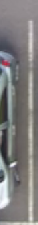
\includegraphics[height=5cm]{secaoMeio}
	\caption{Uma imagem correspondente a uma seção dividida entre carro e vaga vazia, cuja classificação se beneficia do ajuste pelas vizinhas.}
	\label{fig:secaoMeio}
	\centering
\end{figure}

\begin{figure}
	\centering
	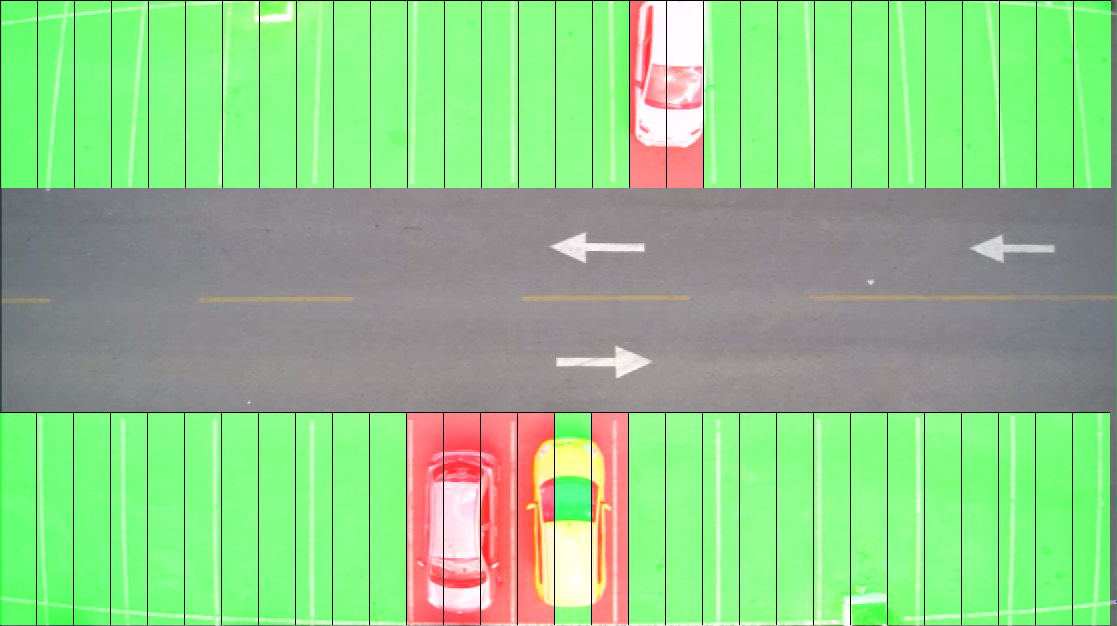
\includegraphics[width=8cm]{erroMeio}
	\caption{Um tipo de erro que o ajuste gaussiano ajuda a corrigir. As seções vermelhas são ocupadas e as verdes são livres.}
	\label{fig:erromeio}
	\centering
\end{figure}

\subsection{Sistema de votação}\label{sec:votacao}

Além do sistema de classificação momentânea, o programa integra um componente que determina a classe majoritária de uma seção durante um intervalo de tempo. Para o \textit{DVE} uma seção pode estar em um de dois estados: estabilizada ou não-estabilizada. No começo da execução do programa, nenhuma seção está estabilizada. 

\begin{figure}
	\centering
	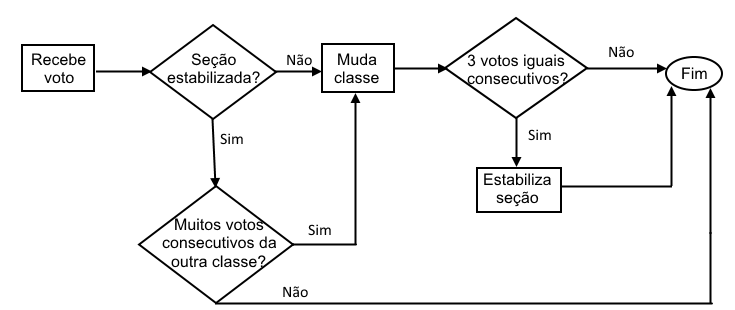
\includegraphics[width=.8\textwidth]{fluxogramaVotos}
	\caption{O fluxograma de funcionamento do sistema de votação.}
	\label{fig:fluxogramaVotos}
	\centering
\end{figure}


Depois de determinar o vetor $y_s$, o sistema determina um voto definido pela Equação \ref{eq:voto}.  Se a seção não estiver estabilizada, sua classe se torna a classe representada pelo voto. Se uma seção receber $3$ votos iguais consecutivamente, a seção se torna estabilizada. Nesse estado, a sua classe não muda mais, mas a seção continua a receber votos. Uma seção deixa de estar estabilizada e volta a poder ser reavaliada se receber um número suficientes de votos consecutivos da classe diferente da sua classe atual ou, mais comumente, quando o \textit{DVE} detecta que houve movimento dentro da área de interesse que intercepta a seção. Esse processo está ilustrado no fluxograma da Figura \ref{fig:fluxogramaVotos}.

Essa etapa do processamento tem o propósito de evitar que flutuações nas imagens das seções causem mudanças frequentes na sua classificação e fazer com que na maioria dos casos a classe de uma seção só mude quando houver movimento detectado na região que ocupada pela seção, trazendo estabilidade para os resultados do programa.

\begin{equation}
voto= 
\begin{cases}
    1,& \text{se } y_s(1) \geq 0,6\\
    2,& \text{caso contrário}
\end{cases}
\label{eq:voto}
\end{equation}


Ao final do processo de classificação, o vetor $v$ de seções é representado visualmente em uma imagem semelhante a Figura \ref{fig:exemploClassificacao}, onde as seções vermelhas são da classe $1$ e representam veículos e as seções verdes são da classe $2$ e representam espaços desocupados.

\begin{figure}
\centering
\includegraphics[width=8cm]{classificada}
\centering
\caption{Um exemplo de quadro com as seções devidamente classificadas, as seções vermelhas representam espaço ocupados por carros, enquanto as verdes representam espaços livres.}
\label{fig:exemploClassificacao}
\end{figure}

\section{Extração do movimento}

Outra ferramenta utilizada pelo \textit{DVE} para a análise do vídeo capturado é a extração do movimento que ocorre na imagem. A cada quadro o programa detecta o movimento ocorrido desde o quadro anterior e processa essa informação para determinar se houve movimento de veículos em alguma das regiões de interesse delimitadas. Mais especificamente, o programa está interessado nos momentos quando um objeto que antes se movimentava termina seu movimento em uma região de interesse ou quando um objeto que iniciou seu movimento dentro de uma ROI finaliza o movimento. Essas situações são entendidas como um veículo estacionando em uma vaga e um veículo sainda de uma vaga respectivamente.

\subsection{Magnitudes do movimento}

O movimento é detectado através do método de cálculo do fluxo óptico utilizando o método de Lucas-Kanade\cite{bruhn2005lucas,faria1992fluxo,mota2011tensor} para resolver a Equação \ref{eq:fluxo2}. O resultado deste processo é uma matriz $M$ de dimensões iguais as do quadro onde cada elemento corresponde à magnitude do vetor velocidade do seu movimento. A direção e o sentido do vetor velocidade não são de interesse do \textit{DVE}, uma vez só os pontos de início e fim do movimento são relevantes para o processamento. A matriz $M$ então passa por um processo de limiarização, onde cada elemento de magnitude menor do que um limiar $t$ tem seu valor redefinido como $0$. O resultado deste processo é uma matriz que mostra as posições do quadro aonde ocorreu movimento significativo. 



\begin{figure}
\centering
\begin{subfigure}{.5\textwidth}
  \centering
  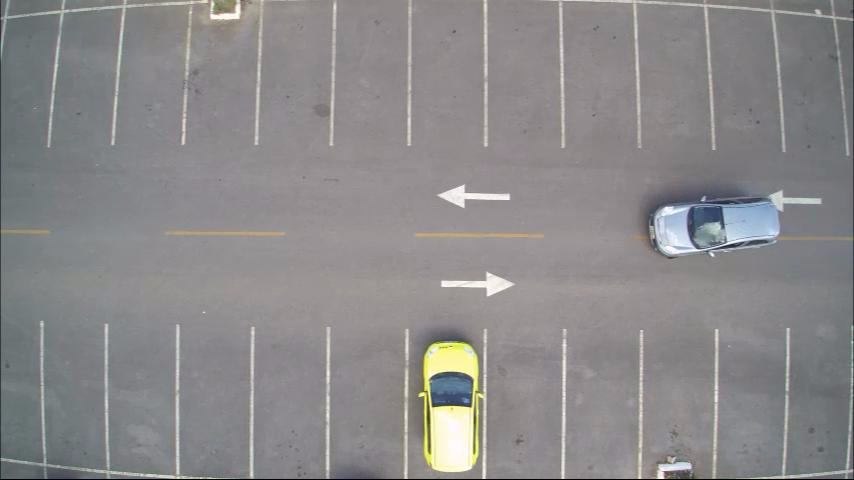
\includegraphics[width=.8\linewidth]{quadroMov}
  \caption{}
  \label{fig:ilustraMovimento:sub:quadro}
\end{subfigure}\\
\begin{subfigure}{.5\textwidth}
  \centering
  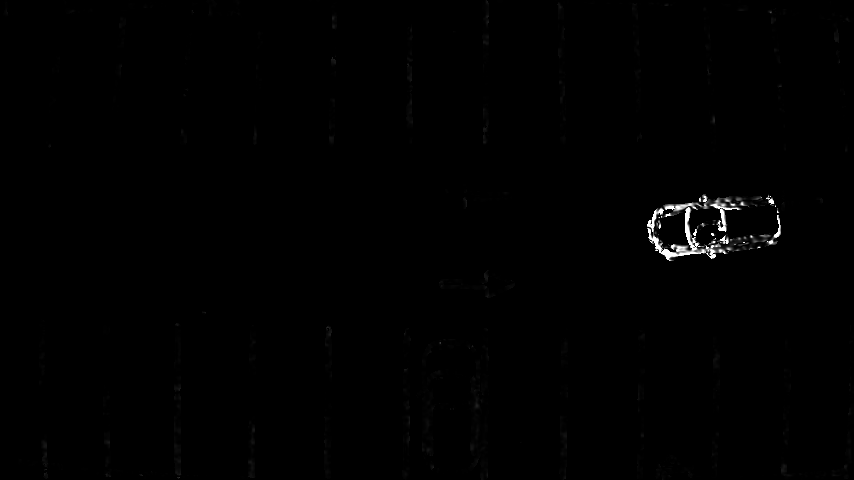
\includegraphics[width=.8\linewidth]{mags}
  \caption{}
  \label{fig:ilustraMovimento:sub:mags}
\end{subfigure}\\
\begin{subfigure}{.5\textwidth}
  \centering
  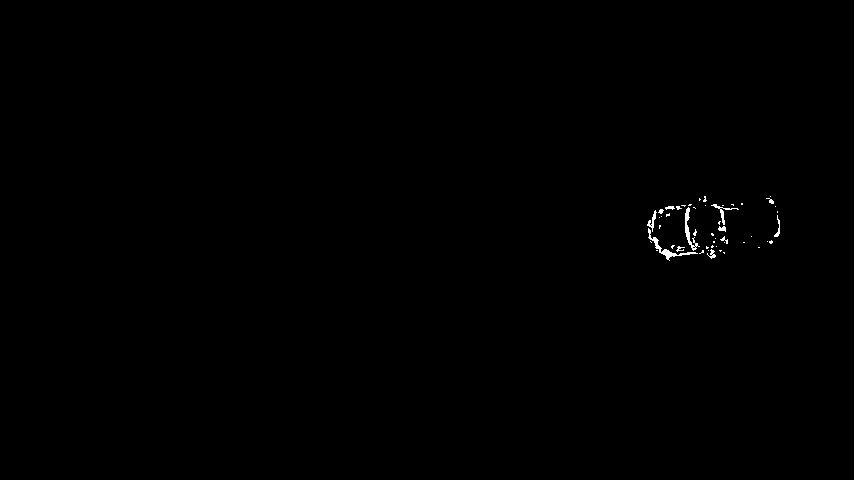
\includegraphics[width=.8\linewidth]{limiarizada}
  \caption{}
  \label{fig:ilustraMovimento:sub:limiarizada}
\end{subfigure}
\centering
\caption{Ilustração do processo de extração do movimento significativo no vídeo. (a) mostra o quadro analisado, (b) uma representação visual da matriz de magnitudes das velocidades e (c) uma representação da matriz depois de limiarizada.}
\label{fig:ilustraMovimento}
\end{figure}


\subsection{Regiões de movimento}\label{sec:sub:regioesmovimento}

Uma vez que a matriz $M$ de magnitudes das velocidades do movimento foi limiarizada, a etapa seguinte é determinar as regiões do quadro que correspondem ao objeto em movimento. Essas regiões são determinadas encontrando pontos na matriz $M$ que correspondem a estimativas dos centros dos objetos móveis, e a partir desses pontos construir um retângulos que representam os limites superiores e inferiores das áreas que os objetos ocupam no quadro.

\begin{equation}
C=\begin{pmatrix}
X_c\\Y_c
\end{pmatrix}
\text{,onde } 
X_c = \frac{\sum_i x_iv_i}{\sum_iv_i}
\text{ e }
Y_c = \frac{\sum_i y_iv_i}{\sum_iv_i}
\label{eq:centros}
\end{equation}

Para se encontrar esses centros, o \textit{DVE} começa separando um vetor $B$ que contém as coordenadas dos pontos diferentes de $0$ de $M$ e os valores destes pontos. A posição do centro de cada objeto em movimento é um vetor de dois elementos onde cada elemento é a média das coordenadas correspondentes dos pontos que compõe o objeto ponderadas pelos valores dos pontos. A Equação \ref{eq:centros} representa esse cálculo, onde $C$ é a posição do centro e $x_i$,$y_i$ e $v_i$ as coordenadas e valores dos pontos que compõe o objeto. A construção dos conjuntos de pontos que representam cada objeto em movimento é feita seguindo os passos abaixo.

\begin{enumerate}
\item Para cada ponto de $B$ faça: 
	\begin{itemize}
		\item Verifique se o ponto está próximo o suficiente de um centro já 				encontrado através da Equação \ref{eq:distancia} de distância.
		\item Caso esteja, associe esse ponto ao conjunto de pontos do objeto e 			recalcule o centro usando a Equação \ref{eq:centros}. 
		\item Caso contrário, inicie um novo conjunto de pontos referente a um 				novo objeto. O centro deste novo conjunto é o ponto.
	\end{itemize}

\item Percorra cada conjunto criado no passo 1 faça e una todos os pares de conjuntos que possuem centros suficientemente próximos de acorodo com a Equação \ref{eq:distancia};

\item Exclua todos os conjuntos com um número muito pequeno de elementos.

\item Para cada conjunto restante, determine as os elementos com menores e maiores valores nas coordenadas $x$ e $y$ em $B$. Esses pontos representam os limites inferiores e superiores do espaço que cada objeto ocupa no quadro.
\end{enumerate}

\begin{equation}
D = \sqrt{(x_1-x_2)^2+(y_1-y_2)^2}
\label{eq:distancia}
\end{equation}

Munido dos limites da área ocupada por cada objeto em movimento na cena, o programa constrói retângulos que representam uma estimativa da posição desses objetos no quadro. Se $x_{min}$, $x_{max}$, $y_{min}$ e $y_{max}$ são, respectivamente, os valores das menores e maiores coordenadas $x$ e $y$ de um objeto, um retângulo na coordenada $(x_{min},y_{min}$ de largura $x_{max}-x_{min}$ e altura $y_{max}-y_{min}$ é criado. A Figura \ref{fig:retanguloMovimento} mostra um exemplo de uma destes retângulos, representado em azul.

\begin{figure}
\centering
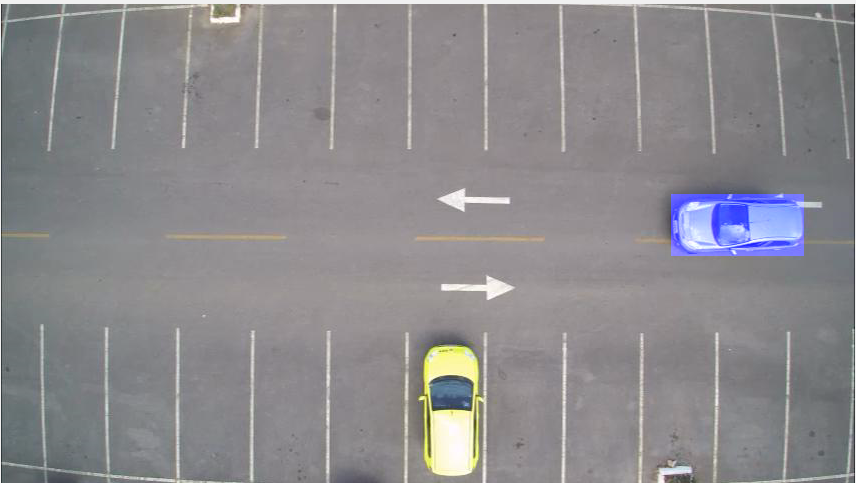
\includegraphics[width=8cm]{retanguloMovimento}
\centering
\caption{Um retângulo que representa a estimativa da área ocupada por um objeto em movimento, representado em azul.}
\label{fig:retanguloMovimento}
\end{figure}

O programa acompanha a posição destes retângulos para determinar o comportamento dos objetos em movimento. O \textit{DVE} armazena a posição inicial de cada retângulo e a sua posição atual. Quando ocorre de um quadro possuir um número menor de retângulos que o anterior, isso significa que o movimento de um objeto se encerrou. Nesse momento, o programa identifica se o início ou o final do movimento encerrado estavam dentro de uma ROI. Se o movimento tiver terminado dentro de uma ROI, as seções interceptadas pelo retângulo referente a sua última posição são reclassificadas. Se o movimento tiver iniciado dentro de uma ROI o mesmo ocorre para as seções interceptadas pelo retângulo referente ao início do movimento. A Figura \ref{fig:movimentoIntercept} ilustra o retângulo interceptando as seções.

\begin{figure}
\centering
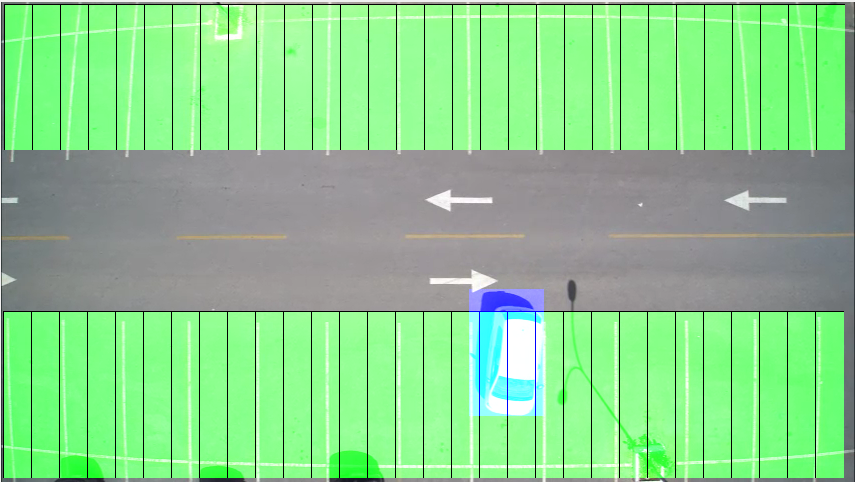
\includegraphics[width=8cm]{retanguloIntercept}
\centering
\caption{O retângulo em azul intereceptando algumas seções verticais. As seções tocadas pelo retângulo serão reclassificadas ao final do movimento.}
\label{fig:movimentoIntercept}
\end{figure}


\section{Mapeamento de Vagas}

Para determinar a quantidade e a posição aproximada das vagas, o programa faz um mapeamento do estacionamento através dos movimentos capturados. Quando um movimento começa ou termina dentro de uma ROI, além de marcar as seções contidas na região deste movimento como não-estabilizadas da forma descrita na Seção \ref{sec:video}, o programa também determina que estas seções compõem uma vaga. Com o tempo, o programa terá determinado quais conjuntos de seções determinam as vagas do estacionamento.

As vagas determinadas desta forma não são estáticas. Na medida que veículos ocupam as seções verticais, as posições das vagas se modificam de acordo com a nova informação. Por exemplo, se uma área de movimento termina sobre duas seções que compõem uma vaga e uma terceira ainda não designada, o programa entende que todas as três seções compõem a mesma vaga. De forma semelhante, se as seções interceptadas por um movimento novo são um subconjunto das seções de uma vaga, estas seções passam a compor uma nova vaga, enquanto a vaga que existia antes passa a ser composta pelas seções restantes. Esse dinamismo permite que erros no mapeamento causados, por exemplo, por veículos mal estacionados ou por alguma falha no próprio programa sejam naturalmente corrigidos com o passar do tempo.

O programa determina que uma vaga foi ocupada se a maioria das seções que a compõem estão classificadas como ocupadas. Por isso, é importante que nenhuma seção pertença a mais de uma vaga. Se isso acontecer, o programa considera a ocupação desta seção mais de uma vez, causando erros na contagem das vagas ocupadas. Além disso, é importante que as seções que compõe uma vaga reflitam o mais corretamente possível, evitando principalmente que duas vagas distintas estejam marcadas na região de uma única vaga. 

Com esses critérios em mente, dois métodos de mapeamento foram desenvolvidos: o modo simples e o modo complexo. No modo simples o programa designa todas as seções interceptadas por um movimento a uma nova vaga, mesmo que essas seções já pertencessem a alguma outra vaga. Apesar de garantir a que nenhuma seção fará parte de duas vagas simultaneamente, essa simplificação traz a desvantagem de ocasionalmente determinar vagas que não refletem corretamente os movimentos. A mais comum destas eventualidades é a criação de vagas compostas de apenas uma seção, exemplificada na Figura \ref{fig:umasecao}. Essas vagas oferecem um risco de erro, uma vez que basta que a seção seja classificada como ocupada para que a vaga também o seja, diminuindo a precisão da consideração. Porém, um novo movimento que intercepte esta seção normalmente a integra em uma vaga que melhor reflete a configuração do estacionamento. Este tipo de situação de erro então tem uma probabilidade muito maior de corrigir com o passar do tempo do que uma seção que pertença a duas vagas, além de menos possibilidade de causarem erros na contagem de vagas ocupadas, já que comumente estas seções estão presentes em regiões desocupadas. Esse método é mais adequado quando o programa está executando com um número elevado de seções verticais. Além deste modo exibir melhor performance, o número elevado de seções ajuda a amenizar o problema mencionado.


\begin{figure}%
\centering
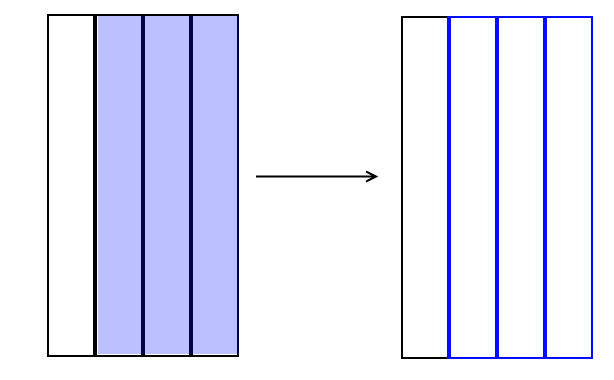
\includegraphics[width=8cm]{umasecao}%
\caption{No quadro a esquerda, um movimento representado pelo retângulo azul intercepta três seções que pertenciam a vaga com os contornos pretos. As seções interceptadas passam a compor uma nova vaga, marcada de azul, enquanto a vaga marcada de preto agora é composta apenas da seção restante.}%
\label{fig:umasecao}%
\centering
\end{figure}

O modo complexo por outro lado segue um conjunto de regras mais elaborado para determinar as vagas a que cada seção pertence. Quando um movimento intercepta um conjunto de seções que chamaremos de $S$, novas vagas são formadas de acordo com os seguintes critérios:

\begin{itemize}
	\item Caso nenhuma seção de $S$ esteja associada a alguma vaga, $S$ passa a compor uma nova vaga.
	\item Caso as seções de uma certa vaga $V$ sejam um subconjunto de $S$, $V$ passa a ser composto por $S$.
	\item Caso $S$ seja um subconjunto de uma vaga $V$, uma nova vaga com as seções de $S$ é criada. Caso as seções de $V$ que não pertenciam a $S$ formem um conjunto contínuo com número de seções suficientemente grande, uma segunda vaga $V_2$ é criada.
	\item Caso a intersecção entre as seções de $S$ e de uma outra vaga $V$ seja não-nula e nenhum dos casos anteriores ocorra, as seções da intersecção são divididas entre as duas vagas. Se houver um número ímpar de seções a dividir, $S$ recebe a seção sobresalente.
\end{itemize}

Esse modo de mapeamento não garante naturalmente que as seções pertençam a uma única vaga, apesar da ocorrência ser rara. Porém, as vagas criadas através deste modo representam melhor a configuração real do estacionamento. Ao contrário do método simples, este modo de mapeamento é mais adequado quando o número de seções verticais em cada área de interesse é menor.

Independentemente do modo escolhido para a execução, o programa determina as vagas no momento inicial do vídeo de forma diferente do que durante o resto da execução. Como neste momento não há movimento algum, as posições das vagas são determinadas apenas pela ocupação das seções verticais. Cada conjunto de seções verticais consecutivas classificadas como ocupadas configuram uma vaga.







